\subsection{GSI}

Для заполнения пропущенных кадров в траектории часто используется метод интерполяции, востребованный благодаря простоте реализации. Однако его точность ограничена отсутствием использования информации о движении, играющем огромную роль в видео с беспилотных летательных аппаратов. В связи с этим рассматривается интерполяционная модель GSI, использующая регрессию на основе гауссовского процесса \cite{8-1}.

Для $i$-ой траектории модель строится следующим образом:
\begin{equation*}
    p_t = f^{(i)}(t)+\epsilon,
\end{equation*}
где $t \in F$ -- номер кадра, $p_t \in P$ -- координаты положений в кадре $(x, y, w, h)$ и $\epsilon \sim N(0, \sigma^2)$ -- гауссовский шум.

Располагая полученными после трекинга и интерполяции траекториями $S^{(i)}={t^{(i)}, p^{(i)}_t}^L_{t=1}$ длины L, задача моделирования нелинейного движения решается путем определения функции $f^{(i)}$. Предполагается, что она описывается гауссовским процессом:

\begin{equation}
    f^{(i)} \in GP(0, k(\cdot, \cdot)),
\end{equation}

\noindent где $k(x, x')=exp(- \frac{||x-x'||^2}{2 \lambda^2})$ -- ядро радиальной базисной функции.

В результате получения множества кадров $F^*$, согласно свойствам гауссовских процессов, сглаженные координаты $P^*$ определяются следующим образом:

\begin{equation}
    P^*=K(F^*,F)(K(F,F) + \sigma^2 I)^{-1}P,
\end{equation}

\noindent где $K(\cdot, \cdot)$ -- функция ковариации для $k(\cdot, \cdot)$.

Наряду с этим существует гиперпараметр $\lambda$, отвечающий за степень гладкости траектории, связанный с ее длиной. Из данных соображений определена следующая функция:

\begin{equation}
    \lambda = \tau \cdot \log{\tau^3 / l},
\end{equation}

\noindent где $\tau$ задается по умолчанию равным 10 по результатам экспериментов.

На Рис. \ref{img:8-1} представлено сравнение GSI, линейной интерполяции и необработанной траектории. Полученные в результате трекинга данные обычно содержат в себе неустойчивый характер шума, тогда как линейная интерполяция игнорирует информацию о движении. Для устранения данных помех модель GSI применяет сглаживание всей траектории при участии контролирующего параметра.

\begin{figure}[ht]
    \centering
    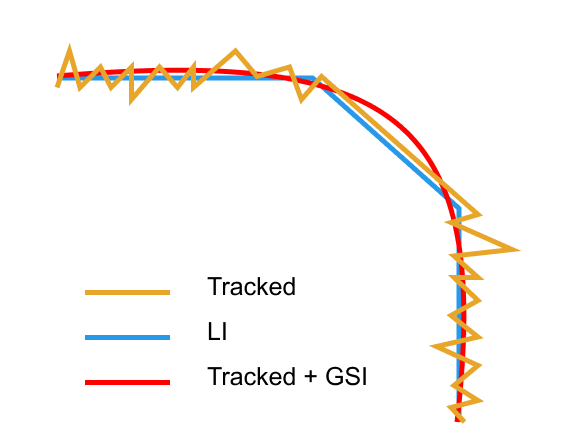
\includegraphics[width=0.85\textwidth]{8-1}
    \caption{Сравнение необработанной траектории (Tracked),\\ линейной интерполяции (LI)\\ и интерполяции с гауссовским сглаживанием (Tracked + GSI)}
    \label{img:8-1}
\end{figure}
